\documentclass[compress,xcolor=table]{beamer}

\usepackage[french]{babel}
\selectlanguage{french}
\usepackage[utf8]{inputenc}
\usepackage[T1]{fontenc}
\usepackage{datetime}
\usepackage[backend=bibtex,style=draft,sorting=debug]{biblatex}
\bibliography{biblio}
\let\stdcite\cite
\renewcommand{\cite}[1]{[\stdcite{#1}]}

\usetheme{stim}

\title{\LARGE Réseaux de Neurones Récurrents\newline{\Large \em Recurrent Neural Networks (RNN)\newline~}}
\foottitle{Réseaux de Neurones Récurrents}
\subtitle{\large Projet de Traitement de l'Écrit}
\date{\formatdate{20}{2}{2015}}
\author{\texttt{G4E} \and Thomas \textsc{Robert}}
\institute{Université de Rouen}

% add notes
%\setbeameroption{show notes}  

\begin{document}


\begin{frame}[plain]
	\titlepage
    \setcounter{framenumber}{0}
\end{frame}

\begin{frame}{Sommaire}
	\vspace{.6cm}
	\tableofcontents

\end{frame}

\section{Architectures classiques de RNN}
\subsection{Historique}
\begin{frame}{Historique}
	\begin{itemize}
		\item \textbf{1943 :} Le neurone formel \cite{McCulloch43}
		\newline Une représentation mathématique d’un neurone biologique.
		\item \textbf{1949 :} Loi d'adaptation \cite{Hebb49}
		\item \textbf{1958 :} Le perceptron \cite{Rosenblatt58}
		\item \textbf{1986 :} Le réseau récurrent de Jordan et Elman \cite{Jordan86}
	\end{itemize}
\end{frame}

\begin{frame}{Le neurone formel}
    
    \begin{columns}
        \begin{column}{.55\textwidth}
            \begin{figure}
                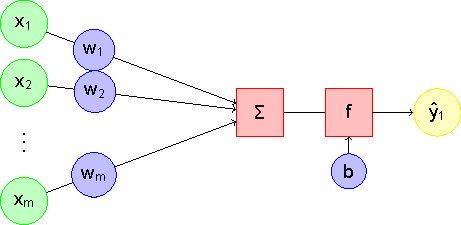
\includegraphics[height=.75\textheight,width=\textwidth,keepaspectratio]{images/neurone}
                \caption{Le neurone formel {\scriptsize\it -- Source : Cours R. \textsc{Hérault} \& P. \textsc{Leray}}}
            \end{figure}
        \end{column}
        \begin{column}{.45\textwidth}
    
            \begin{itemize}
                \item $x_i$ : entrées
                \item $w_i$ : poids
                \item $f$ : fonction d'activation
                \item $b$ : biais
                \item $\hat{y}$ : sortie du neurone
            \end{itemize}
        \end{column}
    \end{columns}
\end{frame}


\subsection{Architectures}
\begin{frame}{Architecture générale}
    \begin{figure}
        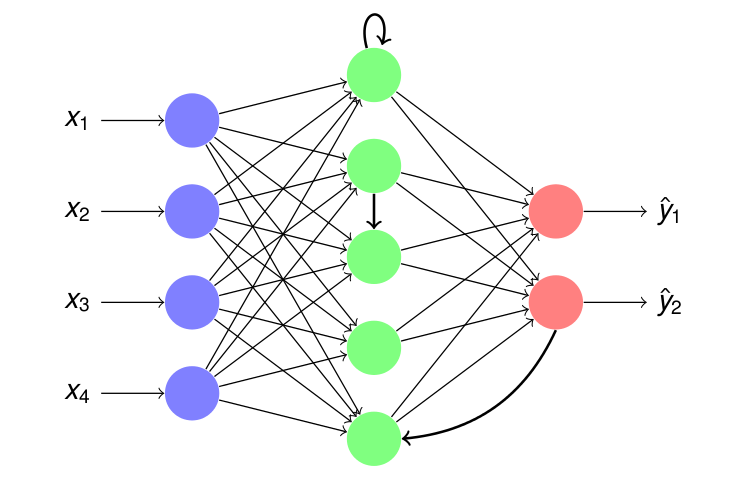
\includegraphics[height=.75\textheight,width=\textwidth,keepaspectratio]{images/arch_rnn_1}
        \caption{Réseau de neurones récurrent {\scriptsize\it -- Source : Cours R. \textsc{Hérault} \& P. \textsc{Leray}}}
    \end{figure}

\end{frame}

\begin{frame}{Architecture d'un RNN d'Elman}
    \begin{figure}
        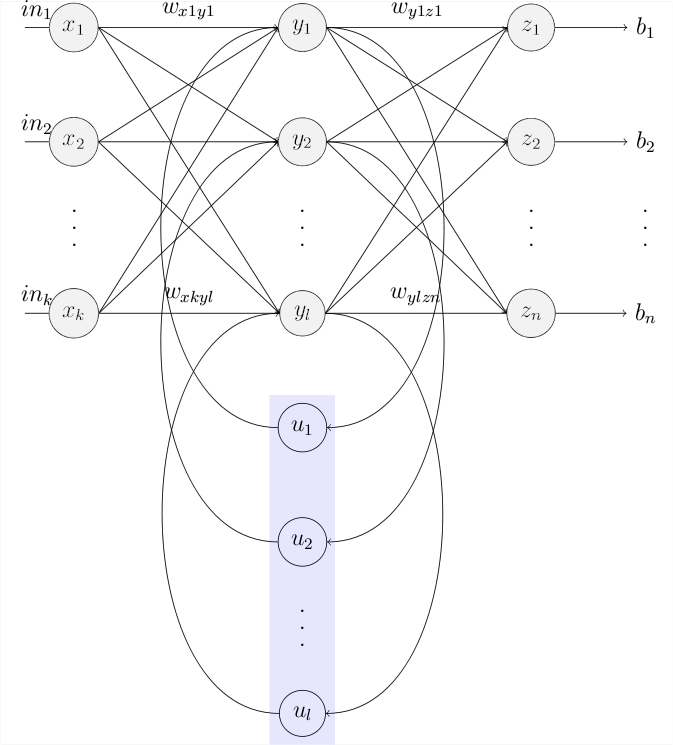
\includegraphics[height=.65\textheight,width=\textwidth,keepaspectratio]{images/Elman_srnn}
        \caption{RNN d'Elman {\scriptsize\it -- Source : wikimedia.org}}
    \end{figure}
    \vspace{-.5cm}
	\begin{itemize} 
		\item La couche $u_1 ... u_n$ sert de mémoire pour l'état précédent 
	\end{itemize}
\end{frame}


\subsection{Apprentissage}
\begin{frame}{Titre de la slide}
	\begin{block}{Texte}
	\begin{itemize}
	\item Item 1
	\end{itemize}
	\end{block}
	
	\begin{alertblock}{Important}
	\begin{itemize}
	\item Item 1
	\end{itemize}
	\end{alertblock}
\end{frame}

\begin{frame}{Titre de la slide}	
	\begin{exampleblock}{Example}
	\begin{itemize}
	\item Item 1
	\end{itemize}
	\end{exampleblock}
	
	\setbeamercolor{block title}{bg=hsrmSec2Dark}
	\setbeamercolor{block body}{bg=hsrmSec2}
	\begin{block}{Autre}
	\begin{itemize}
	\item Item 1
	\end{itemize}
	\end{block}
\end{frame}


\subsection{Applications}
\begin{frame}{Application}
	\begin{itemize}
	\item Très peu d'applications publiées basées sur des RNN simples
		\begin{itemize}
			\item Apprentissage de trajectoires d'espace d'état dans un RNN \cite{Pearlmutter89}
			\item Résolution de l'équation de Sylvester à coefficients variables dans le temps \cite{Zhang02}
			\item Modélisation prosodique du Mandarin et application à la reconnaissance de la parole \cite{Wang02}
		\end{itemize}
	\end{itemize}	

\end{frame}




\section{Nouvelles architectures de RNN}
\subsection{Historique}
\begin{frame}{Motivation}
    \begin{itemize}
        \item Les réseaux de neurones récurrents classiques conservent l'information sur une courte durée (une dizaine d'itérations maximum)
        \item \textbf{1991 :} Démonstration de ce problème par la thèse de Sepp Hochreiter (encadré par Jürgen Schmidhuber) \cite{Hochreiter91}
        \item Recherche de solutions à ce problème par Schmidhuber \& Hochreiter
    \end{itemize}
\end{frame}

\begin{frame}{Apparition des LSTM}
    \begin{itemize}
        \item \textbf{1997 :} \citeauthor{Hochreiter97} publient un article nommé \textit{\citetitle{Hochreiter97}} \cite{Hochreiter97} (fig. \ref{lstm1})
        \item \textbf{2000 :} Ajout de la \og forget gate\fg{} au modèle par \citeauthor{Gers00} \cite{Gers00} (fig. \ref{lstm2})
    \end{itemize}

    \begin{columns}
        \begin{column}{0.48\textwidth}
            \begin{figure}
                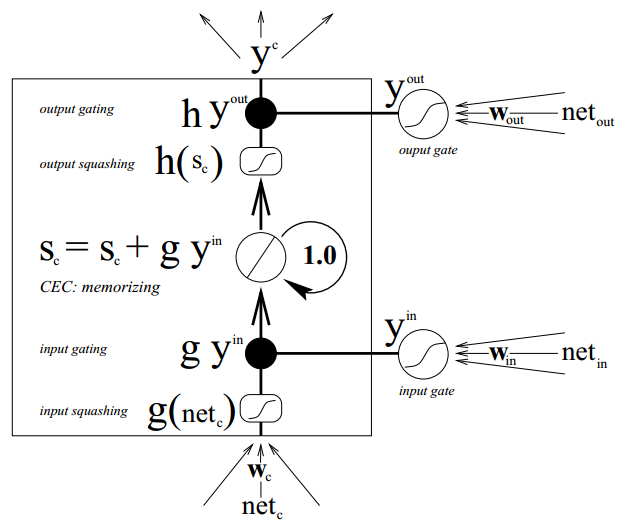
\includegraphics[width=.7\textwidth]{images/lstm1}
                \caption{LSTM orignal}
                \label{lstm1}
            \end{figure}
        \end{column}
        \begin{column}{0.48\textwidth}
            \begin{figure}
                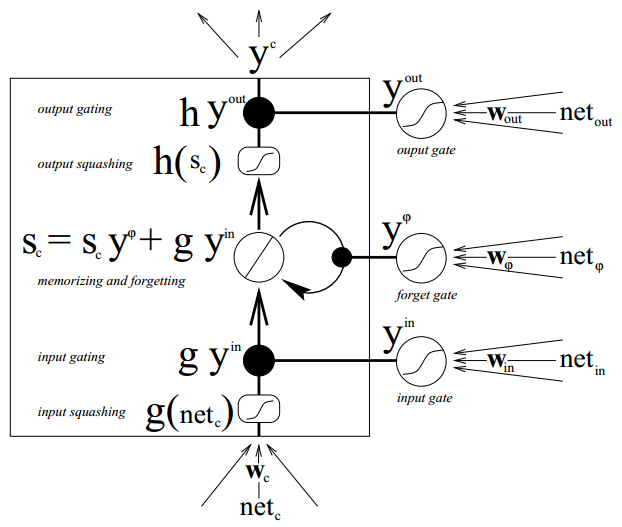
\includegraphics[width=.7\textwidth]{images/lstm2}
                \caption{Ajout de la \og forget gate\fg{}}
                \label{lstm2}
            \end{figure}
        \end{column}
    \end{columns}
\end{frame}

\begin{frame}{Développement des LSTM}
    Le travail sur les LSTM a été poursuivi par Schmidhuber et ses thésards et collaborateurs, en particulier Alex Graves.
    \begin{itemize}
        \item \textbf{2001 :} Apprentissage des langues \cite{Gers01}
        \item \textbf{2003 :} Apprentissage de timings \cite{Gers03}
        \item \textbf{2005 :} Reconnaissance de phonèmes \cite{Graves05a,Graves05b}
        \item \textbf{2006 :} Apprentissage de données non-segmentées \cite{Graves06}
        \item \textbf{2009 :} Reconnaissance de l'écriture \cite{Graves09a,Graves09b}
        \item \textbf{2013 :} Reconnaissance de la parole \cite{Graves13a}
    \end{itemize}
    
    \textbf{Livre de référence :} \citeauthor{Graves12}, \textit{\citetitle{Graves12}} \cite{Graves12}
\end{frame}



\subsection{Architectures}
\begin{frame}{RNN}
    
    \begin{figure}
        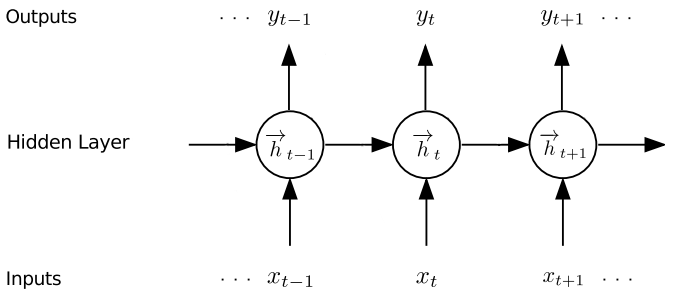
\includegraphics[height=.75\textheight,width=\textwidth,keepaspectratio]{images/arch_rnn}
        \caption{RNN classique {\scriptsize\it -- Source : \cite{Graves13b}}}
    \end{figure}
    
\end{frame}

\begin{frame}{RNN bidirectionnel}
    
    \begin{figure}
        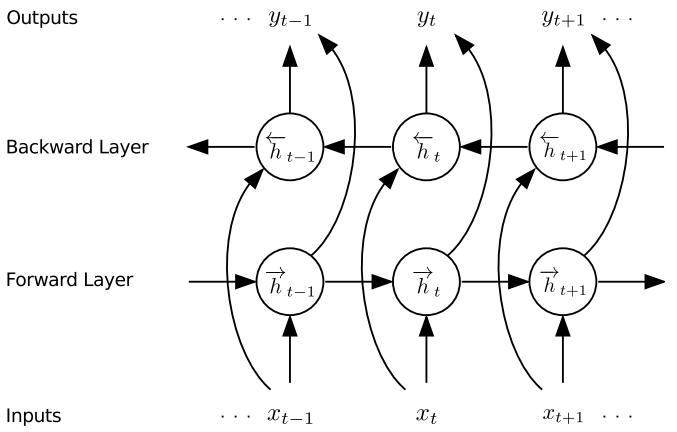
\includegraphics[height=.75\textheight,width=\textwidth,keepaspectratio]{images/arch_brnn}
        \caption{RNN bidirectionnel {\scriptsize\it -- Source : \cite{Graves13b}}}
    \end{figure}
    
\end{frame}

\begin{frame}{RNN bidirectionnel profond}
    
    \begin{figure}
        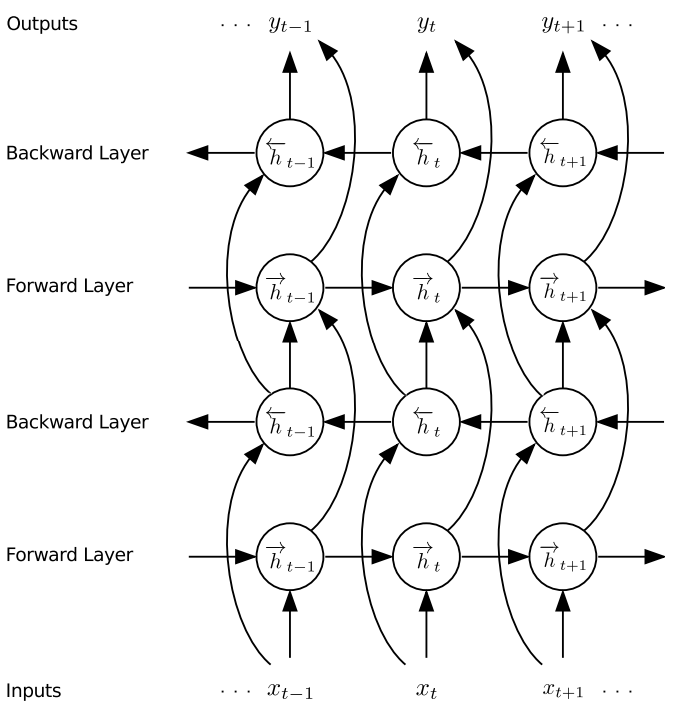
\includegraphics[height=.75\textheight,width=\textwidth,keepaspectratio]{images/arch_dbrnn}
        \caption{RNN bidirectionnel profond {\scriptsize\it -- Source : \cite{Graves13b}}}
    \end{figure}
    
\end{frame}

\begin{frame}{Architecture LSTM}
    
    \begin{figure}
        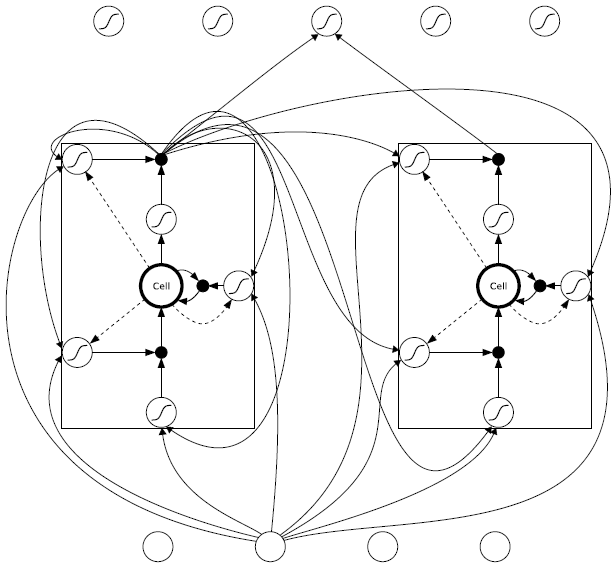
\includegraphics[height=.75\textheight,width=\textwidth,keepaspectratio]{images/arch_lstm}
        \caption{Architecture LSTM {\scriptsize\it -- Source : \cite{Graves12}}}
    \end{figure}
    
\end{frame}

\begin{frame}{LSTM bidirectionnel profond}
    
    \begin{figure}
        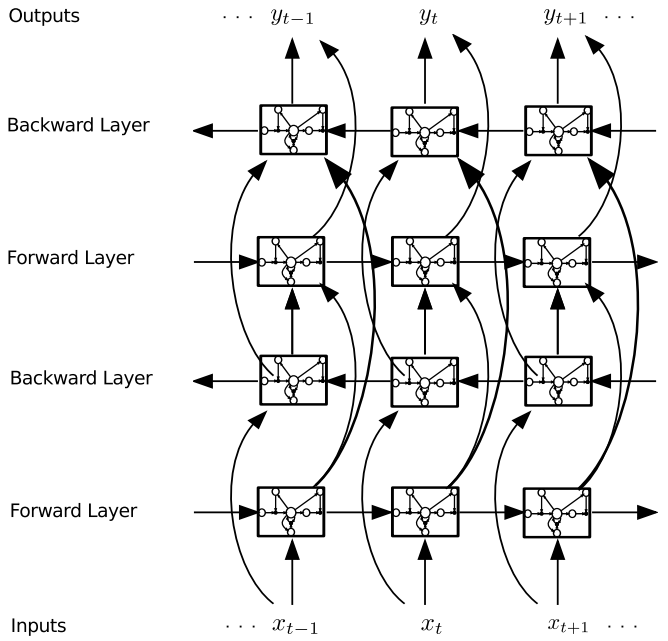
\includegraphics[height=.75\textheight,width=\textwidth,keepaspectratio]{images/arch_dblstm}
        \caption{LSTM bidirectionnel profond (DB-LSTM) {\scriptsize\it -- Source : \cite{Graves13b}}}
    \end{figure}
    
\end{frame}


\subsection{Apprentissage}
\begin{frame}{Apprentissage}
    \begin{itemize}
        \item Utilisation de méthodes d'apprentissage classique adaptées :
            \begin{itemize}
                \item Real Time Recurrent Learning (RTRL) \cite{Robinson87}
                \item BackPropagation Through Time (BPTT) \cite{Williams95}
            \end{itemize}
        \item Possibilité d'approximer le gradient à chaque instant indépendamment des autres avec le RTRL
        \item Possibilité de calculer le gradient exact avec la BPTT \cite{Graves05b}
    \end{itemize}
\end{frame}

\subsection{Applications}
\begin{frame}{Applications}
    \begin{itemize}
        \item Prédiction de la structure de protéines \cite{Sonderby14}
        \item Génération de musique \cite{Eck02}
        \item Reconnaissance de l'écriture \cite{Graves09a,Graves09b}
        \begin{itemize}
            \item Meilleure performance a l'état de l'art. Gain de 3 compétitions à l'ICDAR 2009.
        \end{itemize}
        \item Reconnaissance de la parole \cite{Graves13a,Graves13b}
        \item Reconnaissance d'objets \cite{Ciresan11a}
        \begin{itemize}
            \item Gain de la compétition IJCNN 2011 en reconnaissance de panneaux de signalisation \cite{Ciresan11b}
        \end{itemize}
        \item Etc. {\footnotesize (voir l'interview de Schmidhuber \cite{Angelica12}})
    \end{itemize}
\end{frame}




\section{Conclusion}
\begin{frame}{Conclusion}
    \begin{itemize}
        \item Les réseaux de neurones sont apparus dans les années 1950-60, et les RNN dans les années 1980.
        \item Premiers résultats peu concluants
        \item Regain d'intérêt avec :
        \begin{itemize}
            \item Augmentation de la puissance de calcul
            \item Nouvelles méthodes (Deep Learning, LSTM, ...)
        \end{itemize}
        \item Les LSTM offrent actuellement les meilleures performances à l'état de l'art sur de nombreux problèmes
        \item Méthodes jeunes, peu sorties des labos, recherche active
    \end{itemize}
\end{frame}



\section{Bibliographie}
\begin{frame}[allowframebreaks]{Bibliographie}
%\bibliographystyle{abstract}
%\bibliography{biblio}
\printbibliography
 \end{frame}

\end{document}

